\documentclass[11pt]{article}


\usepackage{amssymb, amsmath, verbatim, amsthm,url, multirow,fullpage,mathtools}
\usepackage{longtable, rotating,makecell,array}
\usepackage[aligntableaux=top]{ytableau}


\setlength{\parindent}{0pt}
\setlength{\parskip}{1.5ex plus 0.5ex minus 0.2ex}


%***************************
%Frontmatter Table of contents
%***************************
% Annotations
%xypic packages
%WLD tkx program
%Useful numeric rings and fields
%Other useful mathematical operations and functions
%Equation display shortcuts
%Shortcuts for frequently used special characters
%Theorem environments
%***************************

%*****************
% Annotations
\usepackage{soul}
\usepackage[colorinlistoftodos,textsize=footnotesize]{todonotes}
\newcommand{\hlfix}[2]{\texthl{#1}\todo{#2}}
\newcommand{\hlnew}[2]{\texthl{#1}\todo[color=green!40]{#2}}
\newcommand{\sanote}{\todo[color=violet!30]}
\newcommand{\note}{\todo[color=green!40]}
\newcommand{\newstart}{\note{The inserted text starts here}}
\newcommand{\newfinish}{\note{The inserted text finishes here}}
\setstcolor{red}
%***************************


%*****************
%xypic packages
\usepackage[all]{xy}
\xyoption{poly}
\xyoption{arc}
%*****************

%*****************
%%% WLD drawing and 2,6 shortcuts

\usetikzlibrary{decorations.pathmorphing,calc}
\usetikzlibrary{intersections}


\definecolor{light-gray}{gray}{0.6}

% some propagator styles
\tikzstyle{propagator}=[decorate,decoration={snake,amplitude=0.8mm}]
\tikzstyle{smallpropagator}=[decorate,decoration={snake,segment length=3mm,amplitude=0.5mm}]

% for highlighting regions of a diagram edge
\tikzstyle{linehighlight}=[red,line width = 3pt,line cap = round, draw opacity = 0.5]

% these two for drawing partial propagators
\tikzstyle{firstdash}=[dashed,line cap=round, dash pattern=on 2pt off 1pt]
\tikzstyle{seconddash}=[dashed,line cap=round, dash pattern=on 0.5pt off 1pt]

% vertices, radius
\newcommand{\drawWLD}[2]{

\pgfmathsetmacro{\n}{#1}
\pgfmathsetmacro{\radius}{#2}
\pgfmathsetmacro{\angle}{360/\n}
\draw (0,0) circle (\radius);
    \foreach \i in {1,2,...,\n} {
      \draw (\angle*\i:\radius) node {$\bullet$};
       %\pgfmathsetmacro{\x}{\angle*\i}
       %\draw[-,shorten >=-\radius*0.1 cm,shorten <=-\radius*0.1 cm]  (\x:\radius cm)-- (\x + \angle: \radius cm);
    }

}

\newcommand{\drawpolypart}[2]{
\pgfmathsetmacro{\n}{#1}
\pgfmathsetmacro{\radius}{#2}
\pgfmathsetmacro{\angle}{360/\n}
    \foreach \i in {1,2,...,\n} {
      \draw (\angle*\i+ \angle/2:\radius) node {$\bullet$};
     \pgfmathsetmacro{\x}{\angle*\i - \angle/2}
      \pgfmathsetmacro{\concave}{((\n-1.5)/\n)}
      \draw (\x:\radius cm) .. controls (\angle *\i: \concave* \radius cm) .. (\x + \angle:\radius cm);
      %\draw (\angle *\i: .8* \radius cm) node {$\bullet$};
    }

}


% r, bumpr, s, bumps: r, s are start/end vertices, bumpr and bumps are how many steps to bump the start/end for multiple props on one edge
\newcommand{\drawprop}[4]{
\pgfmathsetmacro{\r}{#1}
\pgfmathsetmacro{\bumpr}{#2}
\pgfmathsetmacro{\s}{#3}
\pgfmathsetmacro{\bumps}{#4}
\pgfmathsetmacro{\perturbe}{\angle/\n}

\begin{scope}
%\clip (\angle*\r:\radius) -- (\angle + \angle*\r:\radius) -- (\angle*\s:\radius) -- (\angle + \angle*\s:\radius) -- (\angle*\r:\radius);
\draw[smallpropagator] (\angle*\r + \angle/2 + \bumpr*\perturbe:\radius) -- (\angle*\s + \angle/2 + \bumps*\perturbe:\radius);
\end{scope}
}

\newcommand{\drawlabeledprop}[5]{
\pgfmathsetmacro{\r}{#1}
\pgfmathsetmacro{\bumpr}{#2}
\pgfmathsetmacro{\s}{#3}
\pgfmathsetmacro{\bumps}{#4}
\pgfmathsetmacro{\perturbe}{\angle/\n}

\begin{scope}
%\clip (\angle*\r:\radius) -- (\angle + \angle*\r:\radius) -- (\angle*\s:\radius) -- (\angle + \angle*\s:\radius) -- (\angle*\r:\radius);
\draw[smallpropagator] (\angle*\r + \angle/2 + \bumpr*\perturbe:\radius) -- (\angle*\s + \angle/2 + \bumps*\perturbe:\radius) node[midway, below] {#5};
\end{scope}
}


\newcommand{\drawchord}[2]{
\pgfmathsetmacro{\r}{#1}
\pgfmathsetmacro{\s}{#2}

\begin{scope}
%\clip (\angle*\r:\radius) -- (\angle + \angle*\r:\radius) -- (\angle*\s:\radius) -- (\angle + \angle*\s:\radius) -- (\angle*\r:\radius);
\draw (\angle*\r + \angle/2:\radius) -- (\angle*\s + \angle/2:\radius);
\end{scope}
}


% for anything that requires modifying the propagator, e.g. colour, different amplitude,etc
% 5th argument should be {propagator,<other stuff>} or {smallpropagator,<otherstuff>} otherwise you'll get a straight line
\newcommand{\modifiedprop}[5]{
\pgfmathsetmacro{\r}{#1}
\pgfmathsetmacro{\bumpr}{#2}
\pgfmathsetmacro{\s}{#3}
\pgfmathsetmacro{\bumps}{#4}
\pgfmathsetmacro{\perturbe}{\angle/\n}

\begin{scope}
\clip (\angle*\r:\radius) -- (\angle + \angle*\r:\radius) -- (\angle*\s:\radius) -- (\angle + \angle*\s:\radius) -- (\angle*\r:\radius);
\draw[#5] (\angle*\r + \angle/2 + \bumpr*\perturbe:\radius) -- (\angle*\s + \angle/2 + \bumps*\perturbe:\radius);
\end{scope}
}


\newcommand{\boundaryprop}[4]{
\pgfmathsetmacro{\r}{#1}
\pgfmathsetmacro{\bumpr}{#2}
\pgfmathsetmacro{\s}{#3}
\pgfmathsetmacro{\perturbe}{\angle/\n}

\begin{scope}
\clip (\angle*\r:\radius) -- (\angle + \angle*\r:\radius) -- (\angle*\s - \angle:\radius) -- (\angle*\s:\radius) -- (\angle + \angle*\s:\radius) -- (\angle*\r:\radius);
\draw[#4] (\angle*\r + \angle/2 + \bumpr*\perturbe:\radius) -- (\angle*\s:\radius);
\end{scope}
	
}

\newcommand{\drawnumbers}{
  \foreach \i in {1,2,...,\n} {
  \pgfmathsetmacro{\x}{\angle*\i}
  \draw (\x:\radius*1.15) node {\footnotesize \i};
}
}

\newcommand{\drawnumbersshift}{
  \foreach \i in {1,2,...,\n} {
  \pgfmathsetmacro{\x}{\angle*\i + \angle/2}
  \draw (\x:\radius*1.15) node {\footnotesize \i};
}
}



\newcommand{\boundA}[3]{
	\pgfmathsetmacro{\r}{#1}
	\pgfmathsetmacro{\bumpr}{#2}
	\pgfmathsetmacro{\destination}{#3}
	\pgfmathsetmacro{\perturbe}{\angle/\n}
	\path [name path=polyedge1] (\angle*\r:\radius) -- (\angle*\r + \angle:\radius);
	\path [name path=radius1] (0:0) -- (\angle*\r + \angle/2 + \bumpr*\perturbe:\radius);
	\draw[->,
	name intersections={of=polyedge1 and radius1,by=p},
	shorten >=\radius*0.1 cm] (p) ++(\angle*\r + \angle/2 + \bumpr*\perturbe:\radius*0.15) -- (\angle*\destination: \radius*1.15);

}



\newcommand{\boundB}[3]{
	\pgfmathsetmacro{\rangle}{#1*\angle + \angle/2 + #2*\angle/\n}
	\pgfmathsetmacro{\sangle}{#1*\angle + \angle/2 + #3*\angle/\n}


	\draw[->,shorten <=\radius*0.02cm,shorten >=\radius*0.05cm] (\rangle:\radius*1.05) -- (\sangle:\radius*1.05);

}

\newcommand{\makediag}[8]{
	\begin{tikzpicture}[rotate=60,baseline=(current bounding box.east)]
	\begin{scope}
	\drawWLD{6}{0.8}
	%\drawnumbers
	\drawprop{#1}{#2}{#3}{#4}
	\drawprop{#5}{#6}{#7}{#8}
	\end{scope}
	\end{tikzpicture}
}



%%%%%%%
% Drawing partial WLD
%%%%%%%
\def\centerarc[#1](#2)(#3:#4:#5)% Syntax: [draw options] (center) (initial angle:final angle:radius)
    { \draw[#1] ($(#2)+({#5*cos(#3)},{#5*sin(#3)})$) arc (#3:#4:#5); }

\def\clipcenterarc(#1)(#2:#3:#4)% Syntax: [draw options] (center) (initial angle:final angle:radius)
    { \clip ($(#1)+({#4*cos(#2)},{#4*sin(#2)})$) arc (#2:#3:#4); }


%\drawWLDfragment[number of nodes]{radius}{fraction of circle to be displayed}
\newcommand{\drawWLDfragment}[3][10]{
\pgfmathsetmacro{\n}{#1} % use this to get consistent spacing between nodes
\pgfmathsetmacro{\radius}{#2}
\pgfmathsetmacro{\fragment}{#3} % between 0 and 1, gets you that percentage of a circle
\pgfmathsetmacro{\halfangle}{360*\fragment/2}
\pgfmathsetmacro{\startpoint}{270 - \halfangle}
\pgfmathsetmacro{\endpoint}{270 + \halfangle}
\pgfmathsetmacro{\step}{2*\halfangle/\n} 
\pgfmathsetmacro{\zero}{\startpoint-0.5*\step} % so node i is at angle \zero + i*\step
\centerarc[black](0,0)(\startpoint:\endpoint:\radius)
}



\newcommand{\drawnumberspartial}{
\node (0,0) {$\bullet$};
  \foreach \i in {1,2,...,\n} {
  \pgfmathsetmacro{\x}{\step*\i}
  \draw (\zero + \x:\radius*1.15) node {\footnotesize \i};
}
}


\newcommand{\newnode}[3][left]{
	\node[label={[label distance=-1mm]#1:{\scriptsize $#3$}}] at (\zero + #2*\step:\radius) {\scriptsize $\bullet$};
	%\node[#1] at (\zero + #2*\step:\radius) {\scriptsize $#3$};
}

% messier but more flexible: use when you want more control over label placement
\newcommand{\newbetternode}[3][{label distance=-1mm]left}]{
	\node[label={#1:{\scriptsize $#3$}}] at (\zero + #2*\step:\radius) {\scriptsize $\bullet$};
	%\node[#1] at (\zero + #2*\step:\radius) {\scriptsize $#3$};
}



% \newprop[label position]{start node}{end node}{label}
\newcommand{\newprop}[4][midway,below]{
\pgfmathsetmacro{\startnode}{#2}
\pgfmathsetmacro{\endnode}{#3}

\draw[smallpropagator] (\zero+\startnode*\step:\radius) -- (\zero + \endnode*\step:\radius) node[#1] {#4};
}

\newcommand{\newpropbend}[3]{
\draw[smallpropagator] (\zero+#1*\step:\radius*1.1) to[bend left = #3] (\zero + #2*\step:\radius*1.1);
}

%%%%%%%%%%%%%%



%*****************

%*****************
%Useful numeric rings and fields
\newcommand{\Q}{\mathbb{Q}}
\newcommand{\Z}{\mathbb{Z}}
\newcommand{\C}{\mathbb{C}}
\newcommand{\R}{\mathbb{R}}
\newcommand{\N}{\mathbb{N}}
\newcommand{\RP}{\mathbb{R}\mathbb{P}}
\newcommand{\id}{\mathbb{I}}
\newcommand{\Gr}{\mathbb{G}_{\R, \geq 0}}
\newcommand{\Grtnn}{\mathbb{G}_{\R, +}}
\newcommand{\CW}{\overline{\mathcal{W}}} % CW complex of W(k,n)
\newcommand{\BW}{\widehat{\mathcal{W}}} % complex minus bald spots
%*****************


%*****************
%Other useful mathematical operations and functions
\newcommand{\D}{\partial}
\newcommand{\rk}{\textrm{rk }}
\newcommand{\spn}{\textrm{span }}
\newcommand{\rd}{\textrm{d}}
\newcommand{\Res}{\textrm{Res}}
%*****************


%*****************
%Equation display shortcuts
\def\ba #1\ea{\begin{align} #1 \end{align}}
\def\bas #1\eas{\begin{align*} #1 \end{align*}}
\def\bml #1\eml{\begin{multline} #1 \end{multline}}
\def\bmls #1\emls{\begin{multline*} #1 \end{multline*}}
%*****************


%*****************
%Shortcuts for frequently used special characters
\newcommand{\fB}{\mathfrak{B}}
\newcommand{\cP}{\mathcal{P}}
\newcommand{\fZ}{\mathfrak{Z}}
\newcommand{\cM}{\mathcal{M}}
\newcommand{\cA}{\mathcal{A}}
\newcommand{\cI}{\mathcal{I}}
\newcommand{\cC}{\mathcal{C}}
\newcommand{\cB}{\mathcal{B}}
\newcommand{\G}{\mathbb{G}}
\newcommand{\Prop}{\textrm{Prop}}
\newcommand{\cW}{\mathcal{W}}
\newcommand{\bM}{\mathbb{M}}
\newcommand{\cZ}{\mathcal{Z}}
\newcommand{\cY}{\mathcal{Y}}
\newcommand{\Dom}{\textrm{Dom}}
\newcommand{\detzr}[1] {\langle (\cZ_*^\mu|V(p))^{#1} \rangle}
\newcommand{\II}{\mathcal{I}}
\newcommand{\PP}{\mathcal{P}}
\newcommand{\BB}{\mathcal{B}}
\newcommand{\CS}{\mathcal{S}}
\newcommand{\interval}[2]{[\![#1,#2]\!]}
\newcommand{\gale}[1]{\preccurlyeq_{#1}}
\newcommand{\sgale}[1]{\prec_{#1}}
\renewcommand\vec[1]{\overrightarrow{#1}}
\newcommand\cev[1]{\overleftarrow{#1}}
%*****************

%*****************
%Theorem environments
\newtheorem{thm}{Theorem}[section]
\newtheorem{conj}[thm]{Conjecture}
\newtheorem{lem}[thm]{Lemma}
\newtheorem{cor}[thm]{Corollary}
\newtheorem{prop}[thm]{Proposition}
\newtheorem{algorithm}[thm]{Algorithm}


\theoremstyle{remark}
\newtheorem{eg}[thm]{Example}
\newtheorem{claim}[thm]{Claim}

\theoremstyle{definition}
\newtheorem{dfn}[thm]{Definition}
\newtheorem{rmk}[thm]{Remark}
\newtheorem{ntn}[thm]{Notation}
%*****************






\begin{document}





% syntax:

% \drawWLDfragment[number of nodes,optional]{radius}{fraction of circle to be displayed}
% \drawnumberspartial : overlays the number of each node on the diagram to make it easier to code stuff
% \newnode[left/right/etc]{node number}{label (not an optional argument but can be left blank)}
% \newprop[left/right/etc position of label]{start location}{end location}{label}
% \newpropbend{start}{stop}{bend}


% for short propagators that bend, use this template:

% \begin{scope}
% \clipcenterarc(0,0)(\startpoint:\endpoint:\radius)
% \newpropbend{start location}{stop location}{bend in degrees}
% \end{scope}



% Template to set up a partial WLD diagram

% \[
% \begin{tikzpicture}[baseline=(current bounding box.east)]
% 	\begin{scope}
% 	\drawWLDfragment[10]{2}{0.5} 
% 	\drawnumberspartial % use this to debug
% \end{scope}
% \end{tikzpicture}
% \]

% \vspace{4em}
% Working example:

% \[
% \begin{tikzpicture}[baseline=(current bounding box.east)]
% 	\begin{scope}
% 	\drawWLDfragment[8]{4}{0.3} % big radius, small fraction of diagram: wide shallow arc
% 	%\drawnumberspartial
% 	%
% 	% vertices don't get displayed automatically, you have to declare each one that you want to see 
% 	\newnode[above right]{1}{i}
% 	\newnode[below]{2}{i+1}
% 	\newnode[below]{6}{}
% 	%
% 	%
% 	% new propagator: doesn't have to be whole numbers
% 	\newprop[midway,above]{1.5}{8.2}{\footnotesize $p$}
% 	%
% 	%
% 	%
% 	% for small props, we extend them past the edge of the diagram and then clip otherwise they go squiggly at the ends
% 	% so they need to go inside a scope
% 	% \startpoint,\endpoint are the angles that define the start/end of the WLD curve

% 	%
% 	% sometimes we need to place a label manually: the number multiplying the \step corresponds to the numbers in \drawnumberspartial
% 	\node at (\zero + 4.6*\step:\radius*0.9){\footnotesize $q$};
% \end{scope}
% \end{tikzpicture}
% \]

% \newpage 



to replace the currently unlabelled picture in Lemma 3.5 (lem sian)

\[
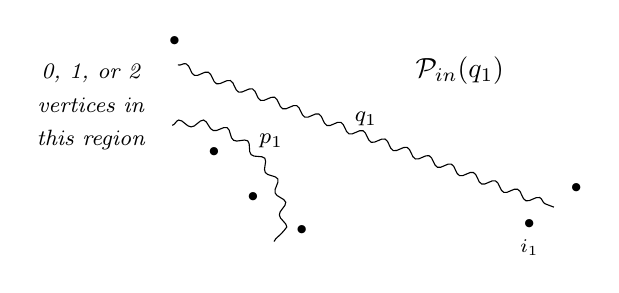
\begin{tikzpicture}[baseline=(current bounding box.east),rotate=-20]
	\begin{scope}
	\drawWLDfragment[10]{3}{0.4} 
	%\drawnumberspartial % use this to debug
	\centerarc[linehighlight](0,0)(\zero + 1.5*\step:\zero + 2.35*\step:\radius)
	\newnode{1}{}
	\newnode{3}{}
	\newnode{4}{}
	\newnode{5}{}
	\newnode[below]{9}{i_1}
	\newnode{10}{}
	\newprop[midway,above]{1.4}{9.5}{\footnotesize $q_1$}
	\begin{scope}
		\clipcenterarc(0,0)(\startpoint:\endpoint:\radius)
		\newpropbend{2.3}{4.7}{60}
		\node at (\zero + 3.5*\step:\radius*0.78) {\footnotesize $p_1$};
	\end{scope}
\node[align = center] at (\zero +1.7*\step:\radius*1.4) {\footnotesize \em 0, 1, or 2 \\ \footnotesize \em vertices in \\ \footnotesize \em this region};
\node at (\zero + 10*\step:\radius*0.3) {$\cP_{in}(q_1)$};

\end{scope}
\end{tikzpicture}
\]


a second picture for lem sian

\[
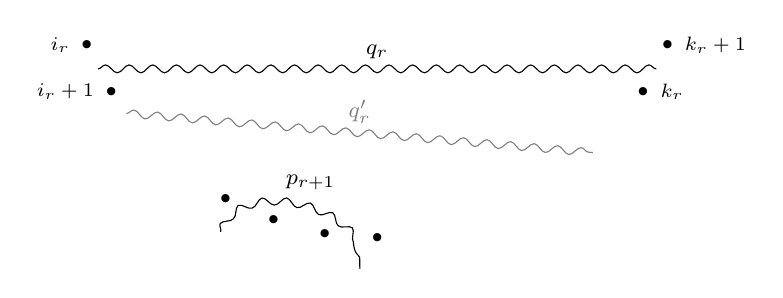
\begin{tikzpicture}[baseline=(current bounding box.east)]
	\begin{scope}
	\drawWLDfragment[15]{4}{0.4} 
	%\drawnumberspartial % use this to debug
	\newnode[left]{1}{i_r}
	\newnode[left]{2}{i_r+1}
	\newnode{5}{}
	\newnode{6}{}
	\newnode{7}{}
	\newnode{8}{}
	\newnode[right]{14}{k_r}
	\newnode[right]{15}{k_r+1}
	\newprop[midway,above]{1.5}{14.5}{\footnotesize $q_r$}
	\draw[smallpropagator,gray] (\zero+2.5*\step:\radius) -- (\zero + 12.5*\step:\radius) node[midway,above,gray] {\footnotesize $q_{r}'$};
	\begin{scope}
		\clipcenterarc(0,0)(\startpoint:\endpoint:\radius)
		\newpropbend{5.2}{7.7}{80}
		\node at (\zero + 6.5*\step:\radius*0.85) {\footnotesize $p_{r+1}$};
	\end{scope}
\end{scope}
\end{tikzpicture}
\]



fig:locally identical

\[
\begin{tikzpicture}[baseline=(current bounding box.east)]
	\begin{scope}
	\drawWLDfragment[12]{3}{0.4} 
	%\drawnumberspartial % use this to debug
	\newnode[left]{1}{i}
	\newnode[below]{4}{j}
	\newnode{5}{}
	\newnode{6}{}
	\newnode{7}{}
	\newnode{8}{}
	\newnode{9}{}
	\newnode{11}{}
	\newnode[right]{12}{l+1}
	\begin{scope}
		\clipcenterarc(0,0)(\startpoint-10:\endpoint+10:\radius)
		\newpropbend{6.3}{8.6}{80}
		\node at (\zero + 7.5*\step:\radius*0.8) {\footnotesize $r$};
		\newprop[midway,left]{5.5}{-4}{}
		\node at (\zero + 3*\step:\radius*0.5) {\footnotesize $p$};
		\newprop[midway]{11.5}{-4}{}
		\node at (\zero + 12.2*\step:\radius*0.7) {\footnotesize $q$};
	\end{scope}
\end{scope}
\end{tikzpicture}
\qquad \qquad
\begin{tikzpicture}[baseline=(current bounding box.east)]
	\begin{scope}
	\drawWLDfragment[12]{3}{0.4} 
	%\drawnumberspartial % use this to debug
	\newnode[left]{2}{m}
	\newnode[below]{4}{j}
	\newnode{5}{}
	\newnode{6}{}
	\newnode{7}{}
	\newnode{8}{}
	\newnode{9}{}
	\newnode{11}{}
	\newnode[right]{12}{l+1}
	\begin{scope}
		\clipcenterarc(0,0)(\startpoint-10:\endpoint+10:\radius)
		\newpropbend{6.3}{8.6}{80}
		\node at (\zero + 7.5*\step:\radius*0.8) {\footnotesize $r$};
		\newprop[midway,left]{5.5}{19}{}
		\node at (\zero + 5.5*\step:\radius*0.5) {\footnotesize $p$};
		\newprop[midway]{11.5}{21}{}
		\node at (\zero + 11.8*\step:\radius*0.8) {\footnotesize $q$};
	\end{scope}
\end{scope}
\end{tikzpicture}
\]





 fig:no fourth vertex

%\draw[smallpropagator,light-gray] (\zero+7.55*\step:\radius*1.1) -- (0:\radius*0.5); 

\[
\begin{tikzpicture}[baseline=(current bounding box.east)]
	\begin{scope}
	\drawWLDfragment[20]{2}{1}
	%\drawnumbers % use this to debug
	\newnode[left]{4}{I_i(p) = i-1}
	\newnode[left]{5}{i}
	\newnode[left]{7}{c}
	\newnode[left]{8}{}
	\newnode[right]{15}{b}
	\newnode[right]{16}{b+1}
	\newprop[midway,above]{4.7}{15.7}{\scriptsize $p$}
	\newprop[midway,below]{7.5}{15.3}{\scriptsize $q$}
      \draw[smallpropagator,light-gray] (\zero +\step *4.3:\radius*1) -- (90:\radius*0.5); 
	\node at (270:\radius*1.5) {\em Case 1};
	% \begin{scope}
	% \clip (\zero + 5*\step:\radius*1.1) rectangle (90:\radius*0.8);
	% \draw[smallpropagator,color=gray] (\zero+4.5*\step:\radius) -- (\zero + 19*\step:\radius);
	% \end{scope}
		\end{scope}
	\end{tikzpicture}
\qquad \qquad 
	\begin{tikzpicture}[baseline=(current bounding box.east)]
	\begin{scope}
	\drawWLDfragment[20]{2}{1}
	%\drawnumbers % use this to debug
	\newnode[left]{4}{a}
	\newnode[left]{5}{}
	\newnode[left]{7}{}
	\newnode[left]{8}{}
	\newnode[right]{15}{b}
	\newnode[right]{16}{b+1 = I_i(p)}
	\newnode[below]{11}{d}
	\newnode[below]{12}{}
	\newnode[above]{2}{i}
	\newprop[midway,above]{4.5}{15.7}{\scriptsize $p$}
		\node at (270:\radius*1.5) {\em Case 2};
	\begin{scope}
	\clip (0,0) circle (\radius);
	%q
	\draw[smallpropagator] (\zero+11.5*\step:\radius*1.2) to [bend left = 45] (\zero + 15.5*\step:\radius*1.2); 
	\node at (\zero + 13.5*\step:\radius*0.55) {\scriptsize $q$};
	%r
	\draw[smallpropagator] (\zero+7.5*\step:\radius*1.2) to [bend left = 45] (\zero + 11.4*\step:\radius*1.2);
	\node at (\zero + 9.5*\step:\radius*0.55) {\scriptsize $r$};

	\end{scope}
		\end{scope}
	\end{tikzpicture}
\] 


 fig V diagram


\[
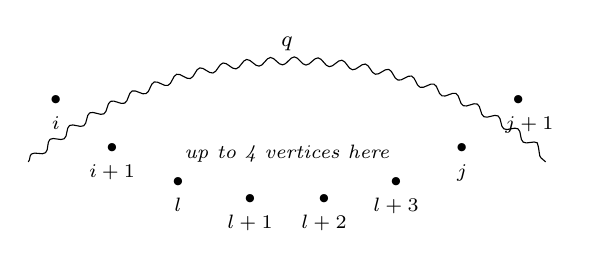
\begin{tikzpicture}[baseline=(current bounding box.east)]
	\begin{scope}
	\drawWLDfragment[8]{4}{0.3}
	%\drawnumbers % use this to debug
	%\clip (\zero + 1.5*\step:1.5*\radius) rectangle (345:{\radius});
	\centerarc[linehighlight](0,0)(\zero + 2.8*\step:\zero + 6.2*\step:\radius)
	\newnode[below]{1}{i}
	\newnode[below]{2}{i+1}
	\newnode[below]{3}{l}
	\newnode[below]{4}{l+1}
	\newnode[below]{5}{l+2}
	\newnode[below]{6}{l+3}
	\newnode[below]{7}{j}
	\newnode[below]{8}{\quad j+1}
	%\node[rotate=-15] at (\zero + 2.7*\step:\radius) {\Large $($};
	%\node[rotate=15] at (\zero + 6.3*\step:\radius) {\Large $)$};
	\node at (\zero + 4.5*\step:\radius*0.85) {\em \scriptsize up to 4 vertices here};
	\begin{scope}
	\clipcenterarc(0,0)(\startpoint-10:\endpoint+10:\radius)
		\draw[smallpropagator] (\zero+1.3*\step:\radius*1.2) to [bend left = 40] (\zero + 7.7*\step:\radius*1.2); 
	\node at (\zero + 4.5*\step:\radius*0.5){\footnotesize $q$};
\end{scope}
\end{scope}
\end{tikzpicture}
\]


 fig special p

\[
\begin{tikzpicture}[rotate = 150,baseline=(current bounding box.east),label distance = -2mm]
\begin{scope}
	\drawWLDfragment[6]{3}{0.3}
	%\drawnumbers % use this to debug
	\begin{scope}
		\clipcenterarc(0,0)(\startpoint:\endpoint:\radius)
		\draw[smallpropagator] (\zero+2.4*\step:\radius*1.1) to [bend left = 55] (\zero + 4.6*\step:\radius*1.1); 
		\node at (\zero + 3.5*\step:\radius*0.75){\footnotesize $p$};
	\end{scope}
	\centerarc[red,line width = 2pt,line cap = round](0,0)(\zero + 2*\step:\zero+4.45*\step:\radius)
	\newbetternode[{[label distance=-3mm]above right}]{1}{n-4}
	\newbetternode[{[label distance=-3mm]above right}]{2}{n-3}
	\newbetternode[{[label distance=-3mm]above right}]{3}{n-2}
	\newbetternode[{[label distance=-3mm]above right}]{4}{n-1}
	\newnode[above]{5}{n}
	\newnode[above]{6}{1}
\end{scope}
\end{tikzpicture}
\qquad 
\qquad 
\begin{tikzpicture}[rotate=150, baseline=(current bounding box.east)]
\begin{scope}
	\drawWLDfragment[7]{3}{0.3}
	%\drawnumbers % use this to debug
	\begin{scope}
		\clipcenterarc(0,0)(\startpoint:\endpoint:\radius)
		\draw[smallpropagator] (\zero+1.4*\step:\radius*1.1) to [bend left = 60] (\zero + 3.5*\step:\radius*1.1); 
		\draw[smallpropagator] (\zero+3.5*\step:\radius*1.1) to [bend left = 60] (\zero + 5.6*\step:\radius*1.1); 
		\node at (\zero + 2.4*\step:\radius*0.8){\footnotesize $q$};
		\node at (\zero + 4.5*\step:\radius*0.8){\footnotesize $p$};
	\end{scope}
	\centerarc[red,line width = 2pt,line cap = round](0,0)(\zero + 1.6*\step:\zero+5.5*\step:\radius)
	\newbetternode[{[label distance=-3mm]above right}]{1}{n-5}
	\newbetternode[{[label distance=-3mm]above right}]{2}{n-4}
	\newbetternode[{[label distance=-3mm]above right}]{3}{n-3}
	\newbetternode[{[label distance=-3mm]above right}]{4}{n-2}
	\newbetternode[{[label distance=-3mm]above right}]{5}{n-1}
	\newnode[above]{6}{n}
	\newnode[above]{7}{1}
\end{scope}
\end{tikzpicture}
\]



 fig 3 cases

Note: check the proof to make sure all the vertices are labeled correctly, since it's been rewritten several times since the picture was drawn, and rewrite any references to ``left two cases'' etc since they now have labels 1, 2, 3, 4.


\begin{tabular}{lll}
% case 1
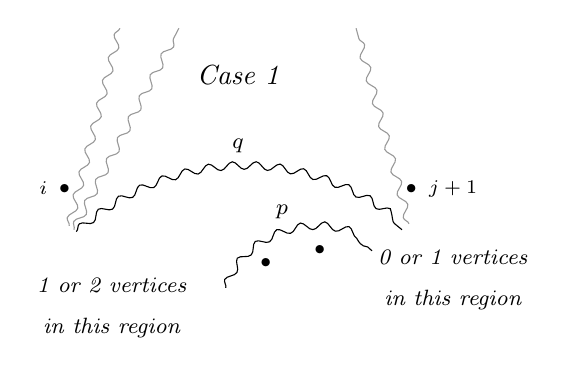
\begin{tikzpicture}[baseline=(current bounding box.east)]
	\begin{scope}
	\drawWLDfragment[8]{3}{0.3} % draws the arc and sets up the parameters
	%\drawnumbers % use this to debug
	% next two lines draw the highlighted regions
	\centerarc[linehighlight](0,0)(\zero + 1.85*\step:\zero + 4.4*\step:\radius)
	\centerarc[linehighlight](0,0)(\zero + 6.75*\step:\zero + 7.4*\step:\radius)
	% labels explaining the highlighted regions
	\node[align = center] at (\zero + 2.7*\step:\radius*1.3) {\em \footnotesize 1 or 2 vertices \\[3pt] \em \footnotesize in this region};
	\node[align = center] at (\zero + 7.5*\step:\radius*1.4) {\em \footnotesize 0 or 1 vertices \\[3pt]\em \footnotesize in this region};
	\begin{scope} % this scope draws the propagators and their labels
		\clipcenterarc(0,0)(\startpoint-20:\endpoint+20:\radius)
		%q
		\draw[smallpropagator] (\zero+1.65*\step:\radius*1.1) to [bend left = 40] (\zero + 7.4*\step:\radius*1.1); 
		%p
		\draw[smallpropagator] (\zero+4.3*\step:\radius*1.1) to [bend left = 55] (\zero + 6.8*\step:\radius*1.1); 
		\draw[smallpropagator,light-gray] (\zero+1.5*\step:\radius*1.1) -- (180:\radius*0.5); 
		\draw[smallpropagator,light-gray] (\zero+1.6*\step:\radius*1.1) -- (180:\radius*0.25);
		\draw[smallpropagator,light-gray] (\zero+7.55*\step:\radius*1.1) -- (0:\radius*0.5); 
		%\draw[smallpropagator,light-gray] (\zero+7.5*\step:\radius*1.1) -- (0:\radius*0.25);  
		\node at (\zero + 4.5*\step:\radius*0.5){\footnotesize $q$};
		\node at (\zero + 5.5*\step:\radius*0.8){\footnotesize $p$};
	\end{scope}
	% draw the nodes
	\newnode[left]{1}{i}
	\newnode[right]{8}{j+1}
	\newnode[below]{5}{}
	\newnode[below]{6}{}
% case label
\node at (270:\radius*0.2) {\em Case 1};
\end{scope}
\end{tikzpicture}
%
%
%
& \qquad \qquad &
%
%
%
% case 2
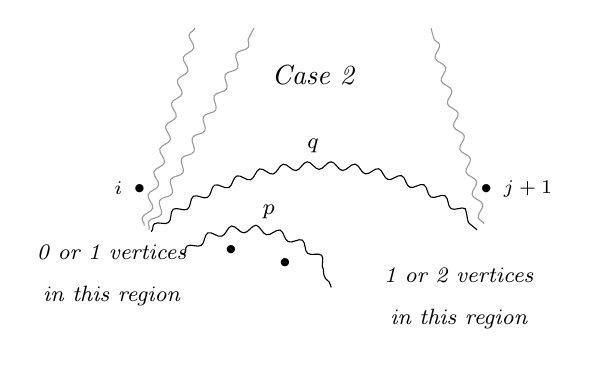
\begin{tikzpicture}[baseline=(current bounding box.east)]
\begin{scope}
	\drawWLDfragment[8]{3}{0.3} % draw arc
	%\drawnumbers % use this to debug
	% highlighted regions
	\centerarc[linehighlight](0,0)(\zero + 1.85*\step:\zero + 2.4*\step:\radius)
	\centerarc[linehighlight](0,0)(\zero + 4.75*\step:\zero + 7.4*\step:\radius)
	%labels for highlighted regions
	\node[align = center] at (\zero + 6.6*\step:\radius*1.3) {\em \footnotesize 1 or 2 vertices \\[3pt]\em \footnotesize in this region};
	\node[align = center] at (\zero + 1.6*\step:\radius*1.35) {\em \footnotesize 0 or 1 vertices \\[3pt]\em \footnotesize in this region};
	% draw props and their labels
	\begin{scope}
		\clipcenterarc(0,0)(\startpoint-20:\endpoint+20:\radius)
		%q
		\draw[smallpropagator] (\zero+1.65*\step:\radius*1.1) to [bend left = 40] (\zero + 7.4*\step:\radius*1.1); 
		%p
		\draw[smallpropagator] (\zero+2.3*\step:\radius*1.1) to [bend left = 55] (\zero + 4.8*\step:\radius*1.1); 
		\draw[smallpropagator,light-gray] (\zero+1.5*\step:\radius*1.1) -- (180:\radius*0.5); 
		\draw[smallpropagator,light-gray] (\zero+1.6*\step:\radius*1.1) -- (180:\radius*0.25);
		\draw[smallpropagator,light-gray] (\zero+7.55*\step:\radius*1.1) -- (0:\radius*0.5); 
		%\draw[smallpropagator,light-gray] (\zero+7.5*\step:\radius*1.1) -- (0:\radius*0.25);  
		\node at (\zero + 4.5*\step:\radius*0.5){\footnotesize $q$};
		\node at (\zero + 3.5*\step:\radius*0.8){\footnotesize $p$};
	\end{scope}
	% nodes
	\newnode[left]{1}{i}
	\newnode[right]{8}{j+1}
	\newnode[below]{3}{}
	\newnode[below]{4}{}
	% case label
	\node at (270:\radius*0.2) {\em Case 2};
\end{scope}
\end{tikzpicture}
%
%
%
\\
\ & \ & \ \\
%
%
%
% case 3
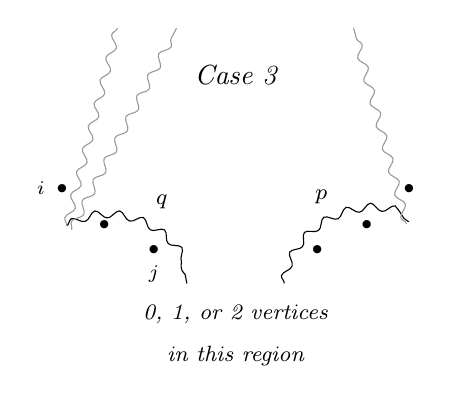
\begin{tikzpicture}[baseline=(current bounding box.east)]
\begin{scope}
	\drawWLDfragment[8]{3}{0.3} % draw arc
	%\drawnumbers % use this to debug
	% highlight region
	\centerarc[linehighlight](0,0)(\zero + 3.6*\step:\zero + 5.4*\step:\radius)
	% region label
	\node[align = center] at (\zero + 4.5*\step:\radius*1.3) {\em \footnotesize 0, 1, or 2 vertices \\[3pt]\em \footnotesize in this region};
	% scope to draw props and their labels
	\begin{scope}
		\clipcenterarc(0,0)(\startpoint-20:\endpoint+20:\radius)
		%q
		\draw[smallpropagator] (\zero+1.5*\step:\radius*1.1) to [bend left = 55] (\zero + 3.7*\step:\radius*1.1); 
		%p
		\draw[smallpropagator] (\zero+5.3*\step:\radius*1.1) to [bend left = 55] (\zero + 7.6*\step:\radius*1.1); 
		\draw[smallpropagator,light-gray] (\zero+1.5*\step:\radius*1.1) -- (180:\radius*0.5); 
		\draw[smallpropagator,light-gray] (\zero+1.6*\step:\radius*1.1) -- (180:\radius*0.25);
		\draw[smallpropagator,light-gray] (\zero+7.55*\step:\radius*1.1) -- (0:\radius*0.5); 
		%\draw[smallpropagator,light-gray] (\zero+7.5*\step:\radius*1.1) -- (0:\radius*0.25);  
		\node at (\zero + 2.8*\step:\radius*0.8){\footnotesize $q$};
		\node at (\zero + 6.5*\step:\radius*0.8){\footnotesize $p$};
	\end{scope}
	% draw nodes
	\newnode[left]{1}{i}
	\newnode[below]{2}{}
	\newnode[below]{3}{j}
	\newnode[below]{6}{}
	\newnode[below]{7}{}
	\newnode[right]{8}{}
	% case label
	\node at (270:\radius*0.2) {\em Case 3};
\end{scope}
\end{tikzpicture}
%
%
%
& \qquad \qquad & \qquad
%
%
%
% case 4
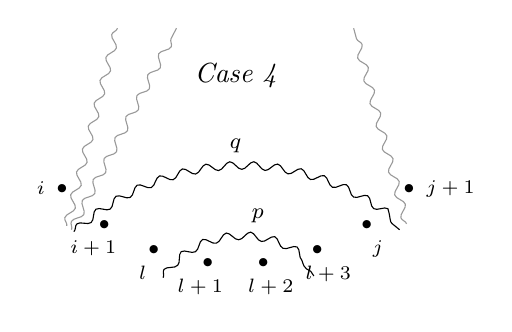
\begin{tikzpicture}[baseline=(current bounding box.east)]
	\begin{scope}
	\drawWLDfragment[8]{3}{0.3} % draw arc
	%\drawnumbers % use this to debug
	%scope to draw props and their labels
	\begin{scope}
		\clipcenterarc(0,0)(\startpoint-20:\endpoint+20:\radius)
		%q
		\draw[smallpropagator] (\zero+1.65*\step:\radius*1.1) to [bend left = 40] (\zero + 7.4*\step:\radius*1.1); 
		%p
		\draw[smallpropagator] (\zero+3.3*\step:\radius*1.1) to [bend left = 55] (\zero + 5.8*\step:\radius*1.1); 
		\draw[smallpropagator,light-gray] (\zero+1.5*\step:\radius*1.1) -- (180:\radius*0.5); 
		\draw[smallpropagator,light-gray] (\zero+1.6*\step:\radius*1.1) -- (180:\radius*0.25);
		\draw[smallpropagator,light-gray] (\zero+7.55*\step:\radius*1.1) -- (0:\radius*0.5); 
		%\draw[smallpropagator,light-gray] (\zero+7.5*\step:\radius*1.1) -- (0:\radius*0.25);  
		\node at (\zero + 4.5*\step:\radius*0.5){\footnotesize $q$};
		\node at (\zero + 5*\step:\radius*0.8){\footnotesize $p$};
	\end{scope}
	% draw nodes
	\newnode[left]{1}{i}
	\newnode[below]{2}{i+1\quad }
	\newnode[below]{3}{l\quad}
	\newnode[below]{4}{l+1\ \ }
	\newnode[below]{5}{\ \ l+2}
	\newnode[below]{6}{\quad l+3}
	\newnode[below]{7}{\quad j}
	\newnode[right]{8}{j+1}
	% case label
	\node at (270:\radius*0.2) {\em Case 4};
\end{scope}
\end{tikzpicture}
\end{tabular}





fig R eg

\begin{tabular}{rrrrr}
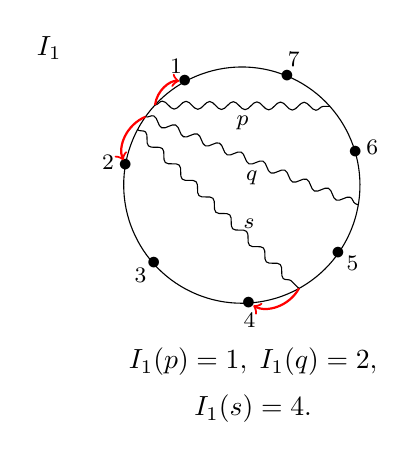
\begin{tikzpicture}[rotate=67.5,baseline=(current bounding box.east)]
	\begin{scope}
	\drawWLD{7}{1.5}
	\drawnumbers
	\drawlabeledprop{1}{-1}{6}{0}{\footnotesize   $p$}
	\drawlabeledprop{1}{0}{5}{0}{\footnotesize   $q$}
	\drawlabeledprop{1}{1}{4}{0}{\footnotesize \; \qquad  $s$}
	\pgfmathsetmacro{\move}{\angle/\n};
	\draw[->,shorten >=2pt,red,thick] (1.5*\angle + -1*\move:\radius) to[bend left = 45] (\angle*1:\radius); %p
	\draw[->,shorten >=2pt,red,thick] (1.5*\angle:\radius) to[bend right = 45] (\angle*2:\radius); %q
	\draw[->,shorten >=2pt,red,thick] (4.5*\angle:\radius) to[bend left = 45] (\angle*4:\radius); %r
	\node at (\angle*1.5:\radius*2) {$I_1$};
	\node[align = center] at (4*\angle:\radius*1.7) {$I_1(p) = 1, \; I_1(q) = 2,$ \\[5pt] $I_1(s) = 4$.};
		\end{scope}
	\end{tikzpicture} 
	& \quad \quad  &
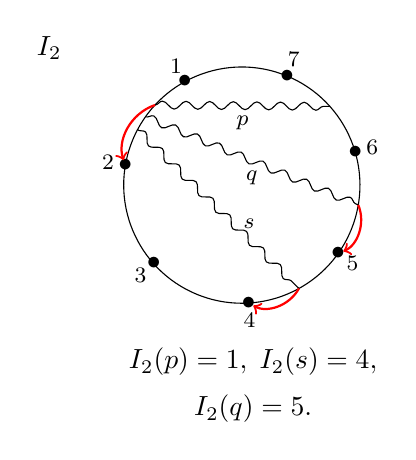
\begin{tikzpicture}[rotate=67.5,baseline=(current bounding box.east)]
	\begin{scope}
	\drawWLD{7}{1.5}
	\drawnumbers
	\drawlabeledprop{1}{-1}{6}{0}{\footnotesize   $p$}
	\drawlabeledprop{1}{0}{5}{0}{\footnotesize   $q$}
	\drawlabeledprop{1}{1}{4}{0}{\footnotesize \; \qquad  $s$}
	\pgfmathsetmacro{\move}{\angle/\n};
	\draw[->,shorten >=2pt,red,thick] (1.5*\angle + -1*\move:\radius) to[bend right = 45] (\angle*2:\radius); %p
	\draw[->,shorten >=2pt,red,thick] (5.5*\angle:\radius) to[bend left = 45] (\angle*5:\radius); %q
	\draw[->,shorten >=2pt,red,thick] (4.5*\angle:\radius) to[bend left = 45] (\angle*4:\radius); %r
	\node at (\angle*1.5:\radius*2) {$I_2$};
	\node[align = center] at (4*\angle:\radius*1.7) {$I_2(p) = 1,  \; I_2(s) = 4,$ \\[5pt] $I_2(q) = 5.$};
	\end{scope} 
\end{tikzpicture}
& \quad & 
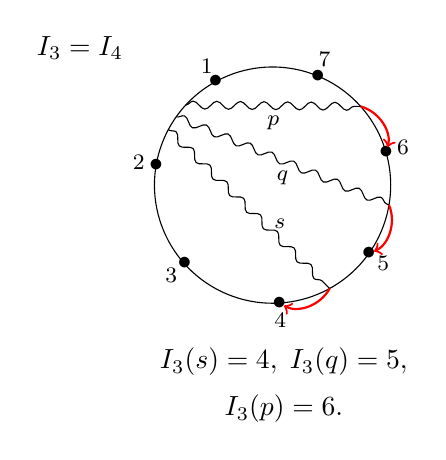
\begin{tikzpicture}[rotate=67.5,baseline=(current bounding box.east)]
	\begin{scope}
	\drawWLD{7}{1.5}
	\drawnumbers
	\drawlabeledprop{1}{-1}{6}{0}{\footnotesize   $p$}
	\drawlabeledprop{1}{0}{5}{0}{\footnotesize   $q$}
	\drawlabeledprop{1}{1}{4}{0}{\footnotesize \; \qquad  $s$}
	\pgfmathsetmacro{\move}{\angle/\n};
	\draw[->,shorten >=2pt,red,thick] (6.5*\angle:\radius) to[bend left = 45] (\angle*6:\radius); %p
	\draw[->,shorten >=2pt,red,thick] (5.5*\angle:\radius) to[bend left = 45] (\angle*5:\radius); %q
	\draw[->,shorten >=2pt,red,thick] (4.5*\angle:\radius) to[bend left = 45] (\angle*4:\radius); %r
	\node at (\angle*1.5:\radius*2) {$I_3 = I_4$};
	\node[align = center] at (4*\angle:\radius*1.7) {$I_3(s) = 4,\;  I_3(q) = 5,$ \\[5pt] $I_3(p) = 6.$ };
	\end{scope} 
\end{tikzpicture}  
\\ 
 & & & &  \\
 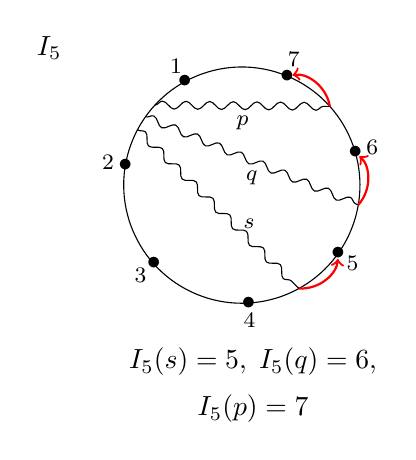
\begin{tikzpicture}[rotate=67.5,baseline=(current bounding box.east)]
	\begin{scope}
	\drawWLD{7}{1.5}
	\drawnumbers
	\drawlabeledprop{1}{-1}{6}{0}{\footnotesize   $p$}
	\drawlabeledprop{1}{0}{5}{0}{\footnotesize   $q$}
	\drawlabeledprop{1}{1}{4}{0}{\footnotesize \; \qquad  $s$}
	\pgfmathsetmacro{\move}{\angle/\n};
	\draw[->,shorten >=2pt,red,thick] (6.5*\angle:\radius) to[bend right = 45] (\angle*7:\radius); %p
	\draw[->,shorten >=2pt,red,thick] (5.5*\angle:\radius) to[bend right = 45] (\angle*6:\radius); %q
	\draw[->,shorten >=2pt,red,thick] (4.5*\angle:\radius) to[bend right = 45] (\angle*5:\radius); %r
	\node at (\angle*1.5:\radius*2) {$I_5$};
	\node[align = center] at (4*\angle:\radius*1.7) {$I_5(s) = 5,\;  I_5(q) = 6,$  \\[5pt] $I_5(p) = 7$ };
	\end{scope} 
\end{tikzpicture}
& \quad & 
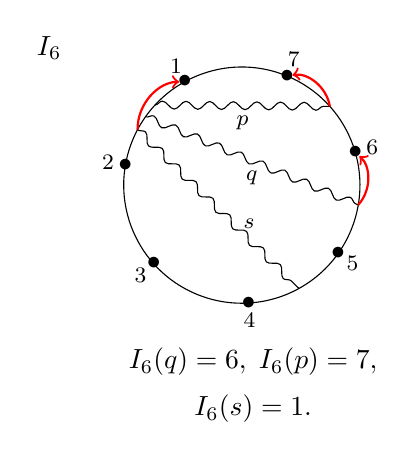
\begin{tikzpicture}[rotate=67.5,baseline=(current bounding box.east)]
	\begin{scope}
	\drawWLD{7}{1.5}
	\drawnumbers
	\drawlabeledprop{1}{-1}{6}{0}{\footnotesize   $p$}
	\drawlabeledprop{1}{0}{5}{0}{\footnotesize   $q$}
	\drawlabeledprop{1}{1}{4}{0}{\footnotesize \; \qquad  $s$}
	\pgfmathsetmacro{\move}{\angle/\n};
	\draw[->,shorten >=2pt,red,thick] (6.5*\angle:\radius) to[bend right = 45] (\angle*7:\radius); %p
	\draw[->,shorten >=2pt,red,thick] (5.5*\angle:\radius) to[bend right = 45] (\angle*6:\radius); %q
	\draw[->,shorten >=2pt,red,thick] (1.5*\angle + 1*\move:\radius) to[bend left = 45] (\angle*1:\radius); %r
	\node at (\angle*1.5:\radius*2) {$I_6$};
	\node[align = center] at (4*\angle:\radius*1.7) {$I_6(q) = 6, \; I_6(p) = 7, $ \\[5pt] $I_6(s) = 1. $ };	
	\end{scope}
	\end{tikzpicture}  
& \quad &
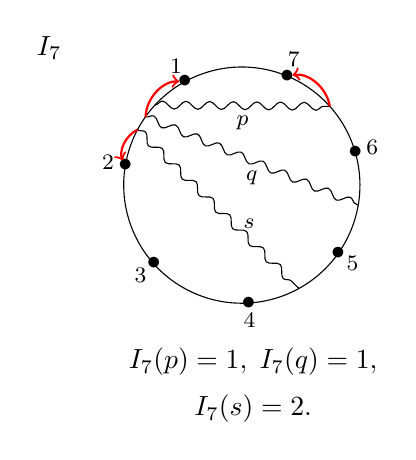
\begin{tikzpicture}[rotate=67.5,baseline=(current bounding box.east)]
	\begin{scope}
	\drawWLD{7}{1.5}
	\drawnumbers
	\drawlabeledprop{1}{-1}{6}{0}{\footnotesize   $p$}
	\drawlabeledprop{1}{0}{5}{0}{\footnotesize   $q$}
	\drawlabeledprop{1}{1}{4}{0}{\footnotesize \; \qquad  $s$}
	\pgfmathsetmacro{\move}{\angle/\n};
	\draw[->,shorten >=2pt,red,thick] (6.5*\angle:\radius) to[bend right = 45] (\angle*7:\radius); %p
	\draw[->,shorten >=2pt,red,thick] (1.5*\angle:\radius) to[bend left = 45] (\angle*1:\radius); %q
	\draw[->,shorten >=2pt,red,thick] (1.5*\angle + \move:\radius) to[bend right = 45] (\angle*2:\radius); %r
	\node at (\angle*1.5:\radius*2) {$I_7$};
	\node[align = center] at (4*\angle:\radius*1.7) {$I_7(p) = 1,  \; I_7(q) = 1, $ \\[5pt] $I_7(s) = 2.$};
	\end{scope} 
\end{tikzpicture}
\\
\end{tabular}





fig no big factors


\[
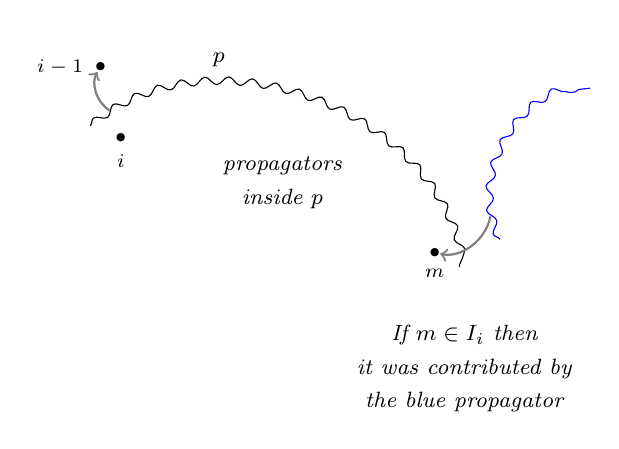
\begin{tikzpicture}[baseline=(current bounding box.east),rotate=-20]
\begin{scope}
	\drawWLDfragment[8]{3}{0.4} 
	%\drawnumberspartial % use this to debug
	\newnode[left]{1}{i-1}
	\newnode[below]{2}{i}
	\newnode[below]{7}{m}
	\begin{scope}
		\clipcenterarc(0,0)(\startpoint-10:\endpoint+10:\radius)
		\newpropbend{1.7}{7.2}{60}
		\draw[smallpropagator,blue] (\zero+7.8*\step:\radius*1.1) to[bend left = 55] (\zero + 10*\step:\radius*1.1);
		\node at (\zero + 1.2*\step:\radius*0.5) {\footnotesize $p$};
	\end{scope}
	\node[align = center,black] at (\zero + \step*4.5:\radius*0.65) {\em \footnotesize propagators \\ \footnotesize \em inside $p$};
	\draw[->,shorten >=2pt,thick,gray] (\zero + 1.6*\step:\radius) to[bend left = 45] (\zero + 1*\step:\radius); %p
	\draw[->,shorten >=2pt,thick,gray] (\zero + 7.9*\step:\radius) to[bend left = 45] (\zero + 7*\step:\radius); 
	\node[align = center,black] at (\zero + 6.8*\step:1.5*\radius) {\em \footnotesize If $m \in I_i$ then \\ \em \footnotesize it was contributed by \\ \em \footnotesize the blue propagator};
\end{scope}
\end{tikzpicture}
\qquad 
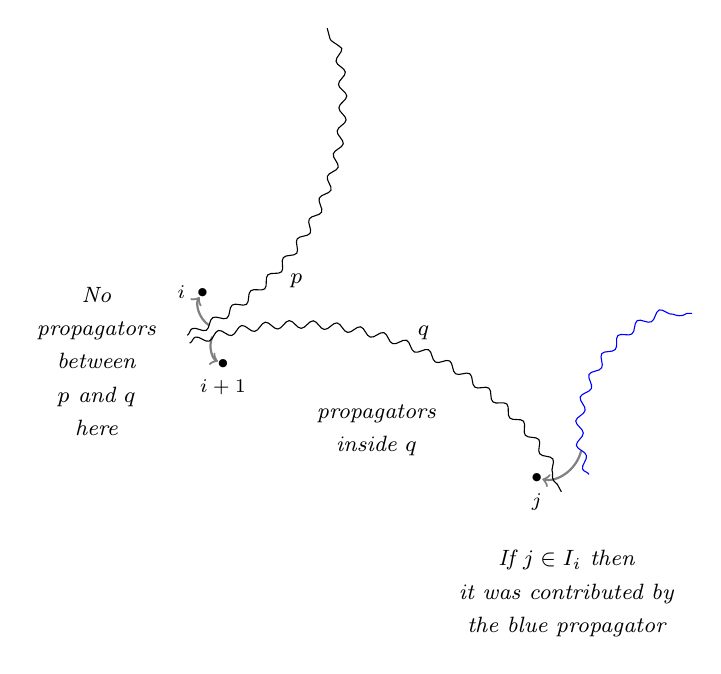
\begin{tikzpicture}[baseline=(current bounding box.east),rotate=-20]
	\begin{scope}
	\drawWLDfragment[8]{3}{0.4}  
	%\drawnumberspartial % use this to debug
	\newnode[left]{1}{i}
	\newnode[below]{2}{i+1}
	\newnode[below]{7}{j}
	\centerarc[red,line width = 2pt,line cap = round](0,0)(\zero + 1.5*\step:\zero+1.56*\step:\radius);
	\draw[->,shorten >=2pt,thick,gray] (\zero + 1.45*\step:\radius) to[bend left = 45] (\zero + 1*\step:\radius); %p
	\draw[->,shorten >=2pt,thick,gray] (\zero + 1.61*\step:\radius) to[bend right = 45] (\zero + 2*\step:\radius); %q 
	\draw[->,shorten >=2pt,thick,gray] (\zero + 7.7*\step:\radius) to[bend left = 45] (\zero + 7*\step:\radius); %blue
	\begin{scope}
		\clipcenterarc(0,0)(\startpoint-10:\endpoint+10:\radius)
		\newpropbend{1.6}{7.2}{40} % q
		\draw[smallpropagator] (\zero+1.5*\step:\radius*1.1) to[bend right = 40] (\zero  - 3*\step:\radius*1.1); % p
		\draw[smallpropagator,blue] (\zero+7.6*\step:\radius*1.1) to[bend left = 55] (\zero + 10*\step:\radius*1.1);
		\node at (\zero + 5*\step:\radius*0.3) {\footnotesize $q$};
		\node at (\zero + 1*\step:\radius*0.6) {\footnotesize $p$};
	\end{scope}
	\node[align = center,black] at (\zero + \step*4.5:\radius*0.75) {\em \footnotesize propagators \\ \footnotesize \em inside $q$};
	\node[align = center] at (\zero + 1.5*\step:\radius*1.5) {\footnotesize \em No \\ \footnotesize \em propagators \\ \footnotesize \em between \\ \footnotesize \em $p$ and $q$ \\ \footnotesize \em here};
	\node[align = center,black] at (\zero + 6.8*\step:1.5*\radius) {\em \footnotesize If $j \in I_i$ then \\ \em \footnotesize it was contributed by \\ \em \footnotesize the blue propagator};
\end{scope}
\end{tikzpicture}
\]




fig quadratic

\[
\begin{tikzpicture}[baseline=(current bounding box.east)]
	\begin{scope}
	\drawWLDfragment[2]{4}{0.1} 
	%\drawnumberspartial % use this to debug
	\newnode[below]{1}{a}
	\newnode[below]{2}{b}
	\begin{scope}
	\clipcenterarc(0,0)(\zero - 1.5*\step:\zero + 4.5*\step:\radius)
	\newprop[midway,left]{1.33}{-7}{\footnotesize $p$}
	\newprop[midway,right]{1.66}{10}{\footnotesize $q$}
	\end{scope}
	\node at (\zero + 0.6*\step:\radius*0.7) {\footnotesize $p$};
	\node at (\zero + 2.4*\step:\radius*0.7) {\footnotesize $q$};
\end{scope}
\end{tikzpicture}
\begin{tikzpicture}[baseline=(current bounding box.east)]
	\begin{scope}
	\drawWLDfragment[2]{4}{0.1} 
	%\drawnumberspartial % use this to debug
	\newnode[below]{1}{b}
	\newnode[below]{2}{a}
	\begin{scope}
	\clipcenterarc(0,0)(\zero - 1.5*\step:\zero + 4.5*\step:\radius)
	\newprop[midway,left]{1.33}{-7}{\footnotesize $q$}
	\newprop[midway,right]{1.66}{10}{\footnotesize $p$}
	\end{scope}
	\node at (\zero + 0.6*\step:\radius*0.7) {\footnotesize $q$};
	\node at (\zero + 2.4*\step:\radius*0.7) {\footnotesize $p$};
\end{scope}
\end{tikzpicture}
\]

fig part4

\[
\begin{tikzpicture}[baseline=(current bounding box.east),rotate = -40]
	\begin{scope}
	\drawWLDfragment[8]{3}{0.4} 
	%\drawnumberspartial % use this to debug
	\newnode{1}{}
	\newnode[left]{2}{i-1}
	\newnode[below]{5}{a-1\quad}
	\newnode[below]{6}{a}
	\newnode[below]{7}{b}
	\begin{scope}
		\clipcenterarc(0,0)(\startpoint:\endpoint+\step:\radius)
		\newpropbend{1.5}{5.7}{20}
		\newpropbend{1.3}{6.4}{30}
		\newprop{6.6}{-6}{}
	\end{scope}
	\node at (\zero + 3.5*\step:\radius*0.8){\footnotesize $s$};
	\node at (\zero + 4.8*\step:\radius*0.45){\footnotesize $p$};
	\node at (\zero + 8*\step:\radius*0.65){\footnotesize $q$};
\end{scope}
\end{tikzpicture}
\]








\end{document}